O diagrama de classes da Figura~\ref{fig:diagrama-classes} modela a estrutura de dados do sistema de certificados com 16 classes distribuídas em módulos funcionais que refletem a separação de responsabilidades definida nos requisitos. Cada classe é identificada por um \texttt{UUID} único, garantindo escalabilidade e independência entre ambientes.

A hierarquia de herança tem como base a classe abstrata \texttt{Pessoa}, que concentra os atributos comuns de identificação (\texttt{id}, \texttt{nome}, \texttt{email}). Dela derivam \texttt{Usuario} e \texttt{Participante}. \texttt{Usuario} representa colaboradores e administradores, com controle de \texttt{perfil} (\texttt{PerfilEnum}), \texttt{ativo}, \texttt{ultimoLogin} e restrição de horários permitidos (\texttt{horarioPermitidoInicio}, \texttt{horarioPermitidoFim}). \texttt{Participante} armazena dados cadastrais como \texttt{cpf}, \texttt{dataCadastro} e status \texttt{ativo}. Essa generalização segue o princípio de herança da orientação a objetos, evitando duplicação de atributos e centralizando a lógica comum de pessoas.

O modelo multi-tenant é implementado pela classe \texttt{Organizacao} (\texttt{nome}, \texttt{cnpj}, \texttt{ativo}), que se associa em cardinalidade \texttt{1} para \texttt{0..*} a \texttt{Usuario}, \texttt{Participante}, \texttt{Curso}, \texttt{Template} e \texttt{Certificado}, e em \texttt{1} para \texttt{1} com \texttt{ConfiguracaoSistema}. Cada organização opera de forma isolada, garantindo que os dados de um inquilino não sejam acessíveis por outro.

A relação entre \texttt{Participante} e \texttt{Curso} é muitos-para-muitos (\texttt{0..*} para \texttt{0..*}), materializada pela classe associativa \texttt{ParticipanteCurso}, que armazena a \texttt{dataVinculo} entre as duas entidades. Essa modelagem foi escolhida por permitir rastrear historicamente quando um participante se vinculou a cada curso, além de facilitar consultas futuras como ``alunos ativos por período''.

No módulo de templates, a classe \texttt{Template} armazena o arquivo com \texttt{nome}, \texttt{tipoArquivo} (\texttt{TipoArquivoEnum}), \texttt{caminhoArquivo}, \texttt{versao}, \texttt{ativo} e \texttt{dataCriacao}. \texttt{CampoDinamico} --- com \texttt{nomeCampo}, \texttt{marcador} e \texttt{tipo} --- modela os marcadores preenchidos na emissão, em composição \texttt{1} para \texttt{0..*} com \texttt{Template}. A assinatura digital é representada por \texttt{AssinaturaDigital} (\texttt{imagemAssinatura}, \texttt{hashVerificacao}, \texttt{dataRegistro}), opcionalmente vinculada ao template (\texttt{1} para \texttt{0..1}).

A classe \texttt{Certificado} é a entidade central do sistema, associada a \texttt{Organizacao}, ao \texttt{Usuario} que o emitiu (relação nomeada \texttt{emitiu}), a \texttt{Participante} (\texttt{0..*} para \texttt{0..*}), a \texttt{Curso} (\texttt{0..*} para \texttt{0..*}) e obrigatoriamente a \texttt{Template} (\texttt{1} para \texttt{1}). Seus atributos incluem \texttt{codigoUnico}, \texttt{dataEmissao}, \texttt{localEmissao}, \texttt{status} (\texttt{StatusCertificadoEnum}), \texttt{arquivoPDF}, \texttt{hashAssinatura} e \texttt{qrCode}. O envio por e-mail é modelado pela classe \texttt{EnvioEmail} (\texttt{status} em \texttt{StatusEnvioEnum}, \texttt{tentativas}, \texttt{dataEnvio}, \texttt{mensagemPersonalizada}), em associação \texttt{1} para \texttt{0..1} com \texttt{Certificado}. A assinatura digital do certificado é vinculada diretamente pela relação \texttt{assinadoCom} entre \texttt{Certificado} e \texttt{AssinaturaDigital} (\texttt{1} para \texttt{1}).

Para auditoria, \texttt{Log} registra eventos genéricos (\texttt{tipo}, \texttt{descricao}, \texttt{dataHora}, \texttt{ip}) vinculados ao usuário (\texttt{1} para \texttt{0..*}), enquanto \texttt{LogAuditoria} armazena ações específicas sobre certificados (\texttt{acao}, \texttt{dataHora}, \texttt{local}), permitindo rastrear quem emitiu ou alterou cada certificado e em qual local.

O suporte técnico é tratado por \texttt{ChamadoSuporte} (\texttt{titulo}, \texttt{descricao}, \texttt{dataAbertura}, \texttt{status} em \texttt{StatusChamadoEnum}, \texttt{dataFechamento}), associado ao usuário que abriu o chamado (relação nomeada \texttt{abriu}) e à organização. As configurações do sistema são centralizadas em \texttt{ConfiguracaoSistema} (\texttt{envioAutomatico}, \texttt{regraReemissao}, \texttt{mensagemPadraoEmail}, \texttt{termosUso}, \texttt{sistemaOnline}), com uma instância por organização (\texttt{1} para \texttt{1}) para controle individualizado de cada inquilino.

\begin{figure}[H]
    \centering
    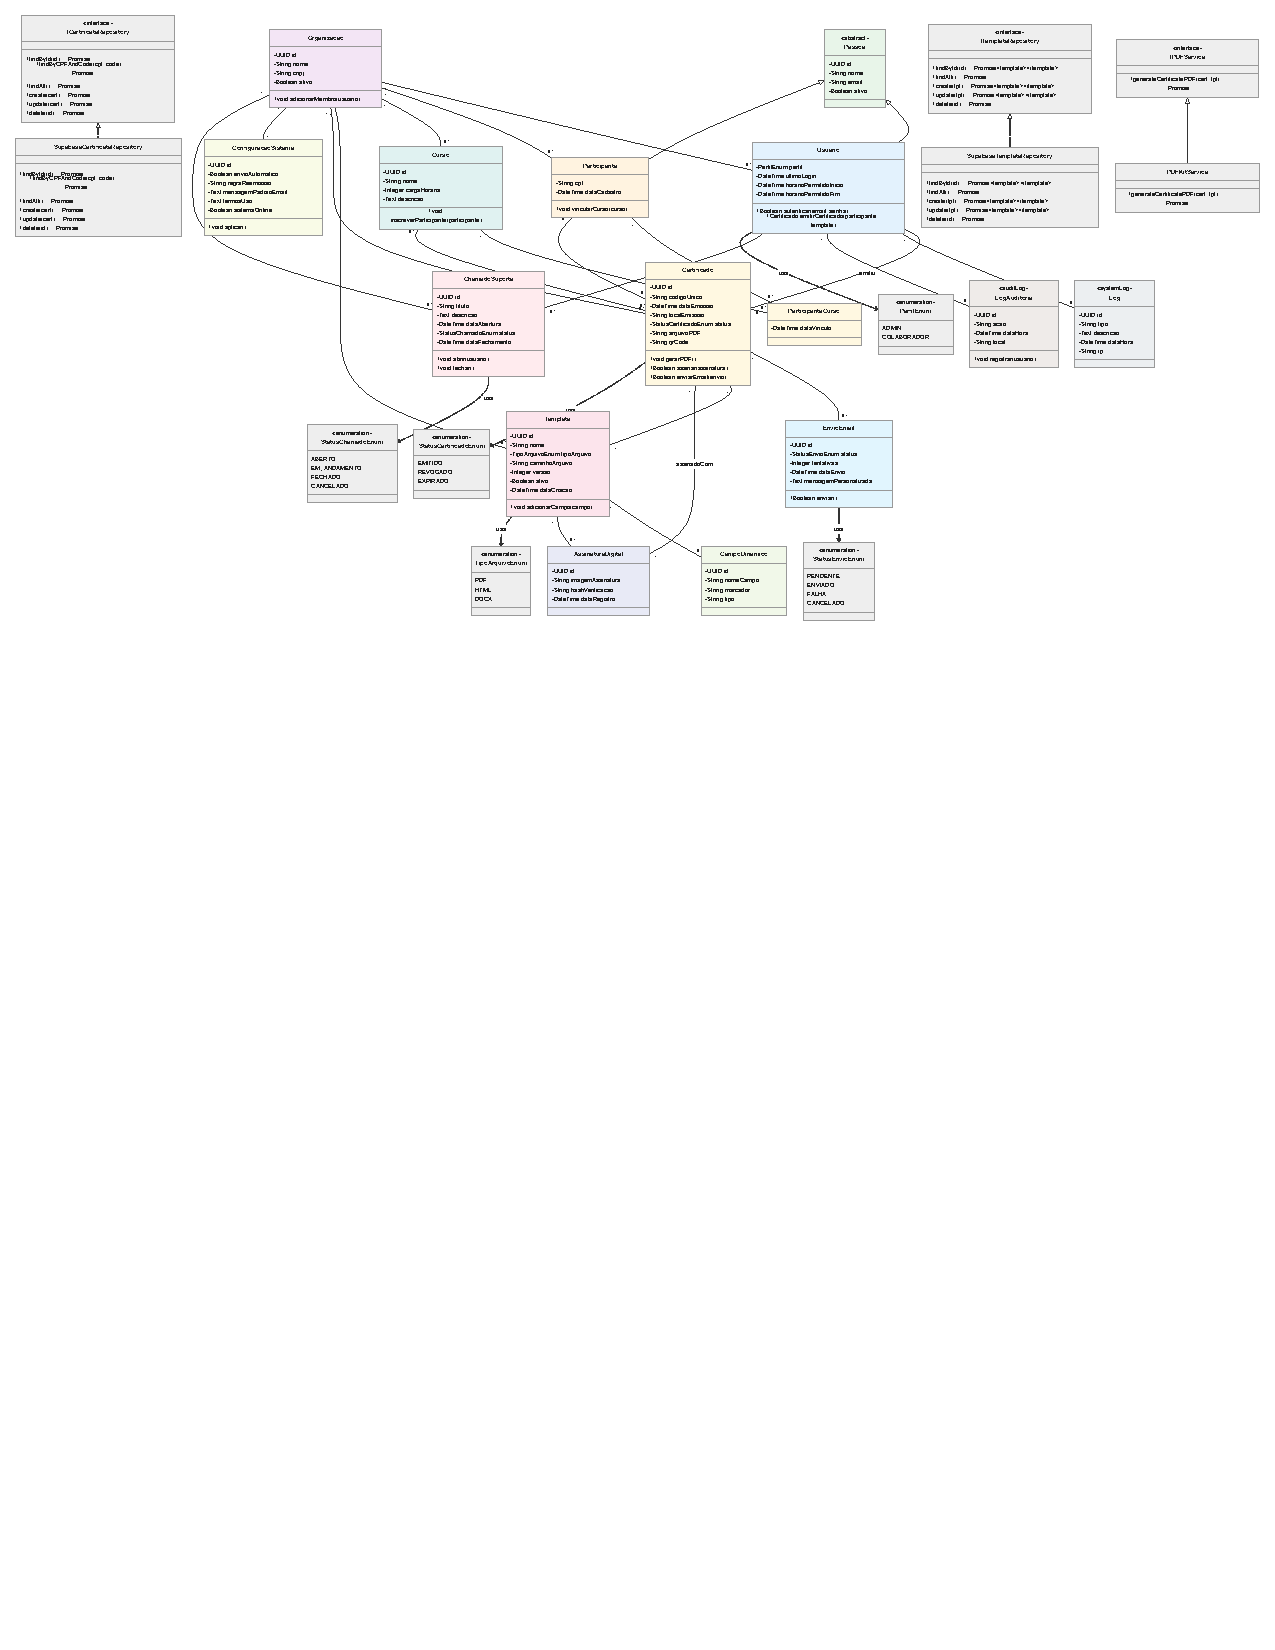
\includegraphics[width=0.9\textwidth]{imagens/diagrama-de-classes.pdf}
    \caption{Diagrama de Classes --- Sistema de Certificados}
    \label{fig:diagrama-classes}
\end{figure}

